%This section provides a description of your product and defines it's primary features and functions. The purpose is to give the document reader/reviewer enough information about the product to allow them to easily follow the specification of requirements found in the remainder of the document. Your header for this section should introduce the section with a brief statement such as: "This section provides the reader with an overview of X. The primary operational aspects of the product, from the perspective of end users, maintainers and administrators, are defined here. The key features and functions found in the product, as well as critical user interactions and user interfaces are described in detail." Using words, and pictures or graphics where possible, specify the following:

This section provides the reader with an overview of the Roam\_Bot. The primary operational aspect of the product for the user is to allow the upload of path finding algorithms for testing. For the maintainers, the primary operational aspects is the functionality of the movement components and crash preventive components, and ensuring hardware is receiving provided algorithms. Key features and functions of the Roam\_Bot are the navigation of a space using the provided algorithm, crash preventative feature, and a simple interface for uploading algorithms.

\subsection{Features \& Functions}
%What the product does and does not do. Specify in words what it looks like, referring to a conceptual diagram/graphic (Figure X).  Define the principle parts/components of the product. Specify the elements in the diagram/graphic that are part(s) of this product as well as any associated external elements (e.g., the Internet, an external web server, a GPS satellite, etc.)
\begin{figure}[h!]
	\centering
    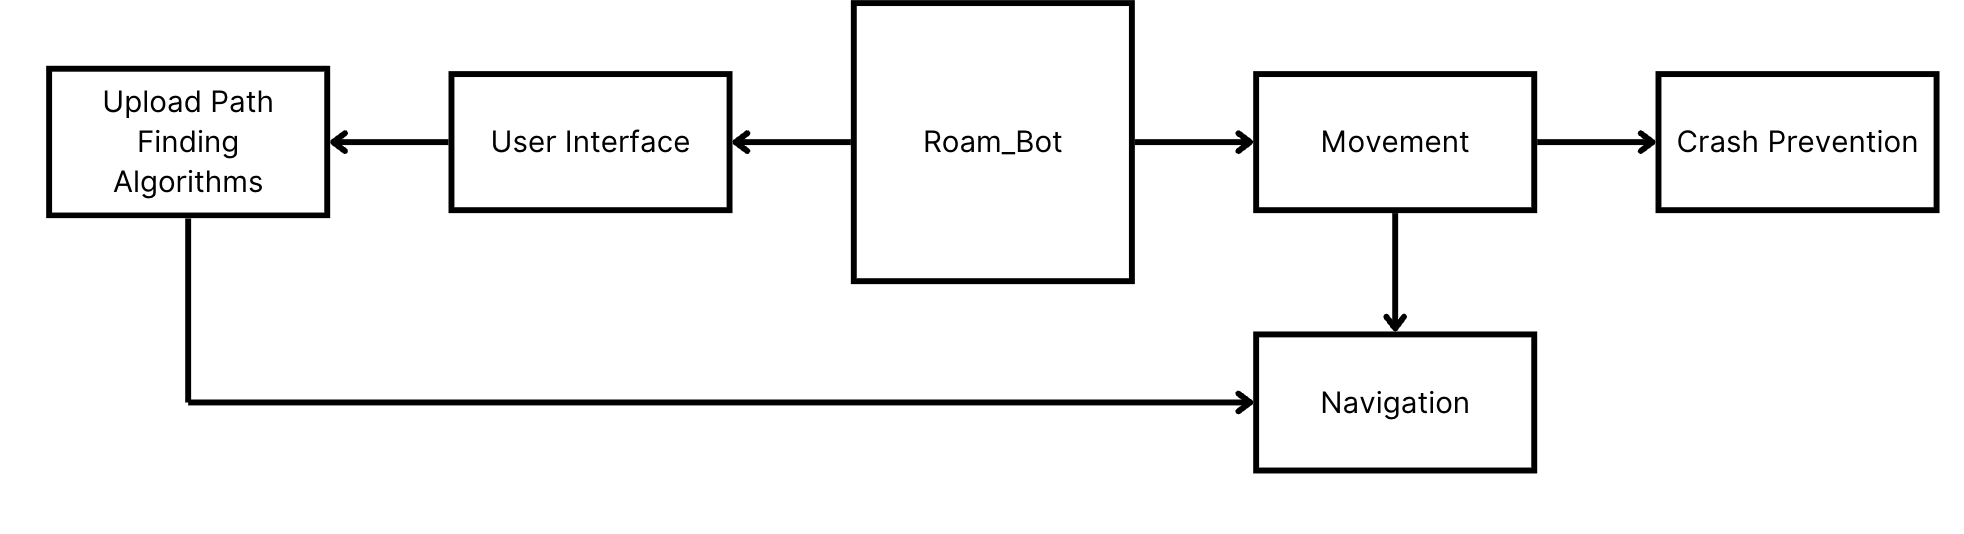
\includegraphics[width=0.90\textwidth]{images/graphic.png} % Change image name
    \caption{Conceptual Diagram of the Roam\_Bot} % Add caption
    \label{fig:conceptual} % Label for referencing
\end{figure}
The Roam\_Bot receives and executes user provided algorithms. The algorithms are uploaded through a simple user interface. Once the start button is pressed the Roam\_Bot will begin navigating using the provided algorithm. The crash prevention feature will ensure that the Roam\_Bot safely avoids collision and navigates away from the obstacle.

\subsection{External Inputs \& Outputs}
%Describe critical external data flows. What does your product require/expect to receive from end users or external systems (inputs), and what is expected to be created by your product for consumption by end users or external systems (outputs)? In other words, specify here all data/information to flow into and out of your systems. A table works best here, with rows for each critical data element, and columns for name, description and use.

\begin{table}[!htbp]
    \centering
    \vspace*{\fill} % Add vertical space to center the table vertically on the page
    \begin{tabular}{| >{\centering\arraybackslash} m{1.5in} | >{\centering\arraybackslash} m{2.5in} | >{\centering\arraybackslash} m{2in} |}
    \hline
     \textbf{Name} & \textbf{Description} & \textbf{Use} \\ \hline
     Uploaded Path finding Algorithm  & The main input that tells the Roam\_Bot how to navigate & The upload is used by users to test algorithms with the Roam\_Bot \\ \hline
     Start Input & This is an input that tells the Roam\_Bot to move & To ensure the Roam\_Bot does not begin moving before it is intended to \\ \hline
     Diagnostic output & Reports the status of internal components & Allows the maintainers to check that the Roam\_Bot is working as expected\\ \hline
    \end{tabular}
    \vspace*{\fill} % Add vertical space after the table for vertical centering
    \caption{Description of the critical external data flows} 
\end{table}


\subsection{Product Interfaces}
%Specify what all operational (visible) interfaces look like to your end-user, administrator, maintainer, etc. Show sample/mocked-up screen shots, graphics of buttons, panels, etc. Refer to the critical external inputs and outputs described in the paragraph above.
The simple user interface will have a simple way for the users to upload their own path finding algorithms, or the option use a default algorithm, and then start the test. The maintainers will see the same user interface but uploading the diagnostic algorithm will create a report on the Roam\_Bots functionality.
